\section{Saules paneļi}
\subsection{Saules paneļa tipa ietekme uz ražīgumu}

Pēc tabulām \ref{tab:JA} un \ref{tab:LG}, kā arī grafikiem, kas integrēti diskusijā par citu saules paneļu parametru efektivitātēm (skat. gada griezumā), redzams, ka LG tipa paneļi konsistenti ir efektīvāki par JA tipu. Tas ir saistīts gan ar kristāla veidu - monokristāliska silīcija paneļi tipiski ir ražīgāki par polikristāliem, % kāda iemesla pēc
gan paneļu maksimālajām jaudām - LG tā ir lielāka nekā JA.

\begin{table}[h]
    \caption{JA tipa paneļu saražotā enerģija uz kvadrātmetru}
    \begin{center}
    %%%%%%%%%%%%%%%%%%%%%%%%%%%%%%%%%%%%%%%%%%%%%%%%%%%%%%%%%%%%%%%%%%%%%%
%%                                                                  %%
%%  This is a LaTeX2e table fragment exported from Gnumeric.        %%
%%                                                                  %%
%%%%%%%%%%%%%%%%%%%%%%%%%%%%%%%%%%%%%%%%%%%%%%%%%%%%%%%%%%%%%%%%%%%%%%
\begin{tabular}{ | c | r r r r r r | } \hline
E, $\textrm{Whm}^{-2}$	&A.13	&R.13	&D.13	&D.40	&D.90	&meteo\\ \hline
jan		&346.66	&227.28	&716.37	&2461.00	&2802.04	&12138.68\\
feb		&3198.12	&2742.33	&4266.63	&6448.71	&5989.95	&25142.93\\
mar		&8222.23	&7397.80	&9472.24	&11938.03	&8717.90	&61764.12\\
apr		&19886.40	&19230.18	&23268.02	&25425.75	&18249.96	&141410.71\\ \hline
$\textrm{E_{sum}}$, $\textrm{kWhm}^{-2}$	&31.7	&29.6	&37.7	&46.3	&35.8	&240.5\\ \hline
\end{tabular}
    \end{center}
    \label{tab:JA}
\end{table}
\begin{table}[h]
    \caption{LG tipa paneļu saražotā enerģija uz kvadrātmetru}
    \begin{center}
    %%%%%%%%%%%%%%%%%%%%%%%%%%%%%%%%%%%%%%%%%%%%%%%%%%%%%%%%%%%%%%%%%%%%%%
%%                                                                  %%
%%  This is a LaTeX2e table fragment exported from Gnumeric.        %%
%%                                                                  %%
%%%%%%%%%%%%%%%%%%%%%%%%%%%%%%%%%%%%%%%%%%%%%%%%%%%%%%%%%%%%%%%%%%%%%%
\begin{tabular}{ | c | r r r r r r | }\hline
E, $\textrm{Whm}^{-2}$	&A.13	&R.13	&D.13	&D.40	&D.90	&piranometrs\\ \hline
jan		&495.5	&347.83	&950.75	&2816.81	&3215.06	&12138.68\\
feb		&4431.55	&3625.5	&5046.58	&8253.64	&7413.21	&25142.93\\
mar		&10916.97	&9267.88	&11271.89	&15694.83	&11337.26	&61764.12\\
apr		&27632.28	&25460.2	&29136.2	&34213.52	&23176.05	&141410.71\\ \hline
$E_{sum}$, $\textrm{kWhm}^{-2}$	&43.5	&38.7	&46.4	&70.0		&45.1	&240.5\\ \hline
\end{tabular}
    \end{center}
    \label{tab:LG}
\end{table}


\subsection{Efektivitāte}

Efektivitāte atšķiras no ražotāju tehniskajā dokumentācijā dotā. Iespējams tāpēc, ka visu paneļu saules apstarojuma references punktu izvēlējos eksperimentālā poligona meteostacijas datus un nepiereizināju tiem panelim atbilstošo leņķi, jo saules apstarojums mainās no leņķa.
% you better do it fast 
\begin{figure}[h]
    \centering
    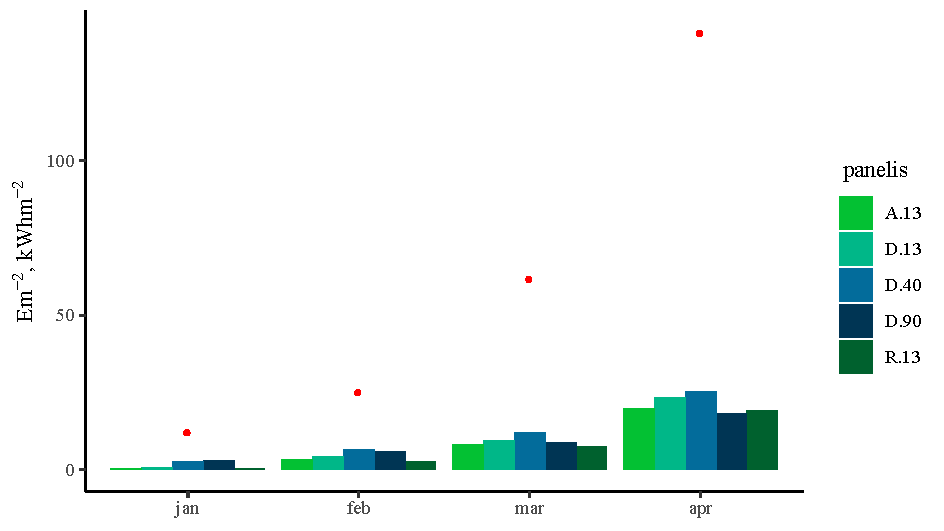
\includegraphics[width=\linewidth]{figures/results/ja_m2.pdf}
    \caption{JA tipa paneļu saražotais mēnesī salīdzinājumā ar eksperimentālā poligona meteostacijas stacijas saules apstarojuma datiem (sarkanā krāsā)}
    \label{fig:ja}
\end{figure}
\begin{table}[h]
    \caption{JA tipa paneļu efektivitāte procentos}
    \begin{center}
    %%%%%%%%%%%%%%%%%%%%%%%%%%%%%%%%%%%%%%%%%%%%%%%%%%%%%%%%%%%%%%%%%%%%%%
%%                                                                  %%
%%  This is a LaTeX2e table fragment exported from Gnumeric.        %%
%%                                                                  %%
%%%%%%%%%%%%%%%%%%%%%%%%%%%%%%%%%%%%%%%%%%%%%%%%%%%%%%%%%%%%%%%%%%%%%%
\begin{tabular}{ | c | c c c c c | } \hline
E, $\%$	&A.13	&R.13	&D.13	&D.40	&D.90\\ \hline
jan	&2.86	&1.87		&5.90	&20.27	&23.08\\
feb	&12.72	&10.91		&16.97	&25.65	&23.82\\
mar	&13.31	&11.98		&15.34	&19.33	&14.11\\
apr	&14.06	&13.60		&16.45	&17.98	&12.91\\ \hline
vid	&10.74	&9.59		&13.67	&20.81	&18.48\\ \hline
\end{tabular}
    \end{center}
    \label{tab:JA_eff}
\end{table}

\begin{figure}[h]
    \centering
    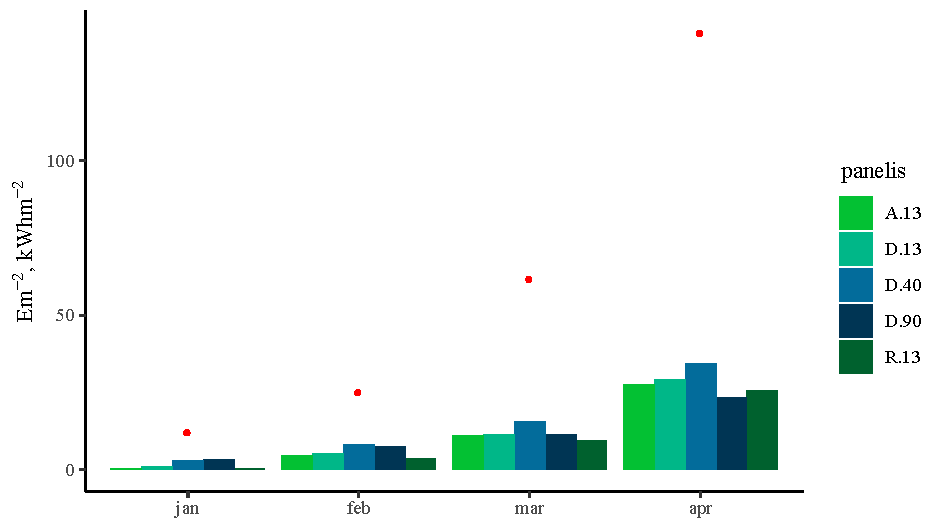
\includegraphics[width=\linewidth]{figures/results/lg_m2.pdf}
    \caption{LG tipa paneļu saražotais mēnesī salīdzinājumā ar eksperimentālā poligona meteostacijas stacijas saules apstarojuma datiem (sarkanā krāsā)}
    \label{fig:lg}
\end{figure}
\begin{table}[h]
    \caption{LG tipa paneļu efektivitāte procentos}
    \begin{center}
    %%%%%%%%%%%%%%%%%%%%%%%%%%%%%%%%%%%%%%%%%%%%%%%%%%%%%%%%%%%%%%%%%%%%%%
%%                                                                  %%
%%  This is a LaTeX2e table fragment exported from Gnumeric.        %%
%%                                                                  %%
%%%%%%%%%%%%%%%%%%%%%%%%%%%%%%%%%%%%%%%%%%%%%%%%%%%%%%%%%%%%%%%%%%%%%%
\begin{tabular}{ | c | c c c c c | }\hline
E, $\%$	&A.13	&R.13	&D.13	&D.40	&D.90\\ \hline
jan		&4.1	&2.9	&7.8	&23.2	&26.5\\
feb		&17.6	&14.4	&20.1	&32.8	&29.5\\
mar		&17.7	&15.0	&18.2	&25.4	&18.4\\
apr		&19.5	&18.0	&20.6	&24.2	&16.4\\ \hline
vid		&14.7	&12.6	&16.7	&26.4	&22.7\\ \hline
\end{tabular}
    \end{center}
    \label{tab:LG_eff}
\end{table}


%%%%%%%%%
\subsection{Saules paneļa leņķa ietekme uz ražīgumu}
Kopumā var secināt, ka 90 grādu leņķi ir ražīgāki ziemas mēnešos un 13 grādu leņķi -- vasaras mēnešos, jo tā paredz Saules diennakts kustības maiņa gada griezumā. Apkopojot četru mēnešu datus un abus paneļu tipus, visražīgākais leņķis ir 40 grādu.
% Tas sakrīt ar [ielikt grafiku ar LV karti un optimālo leņķi bet es neatceros no kurienes paņēmu to].
\begin{figure}[h]
    \centering
    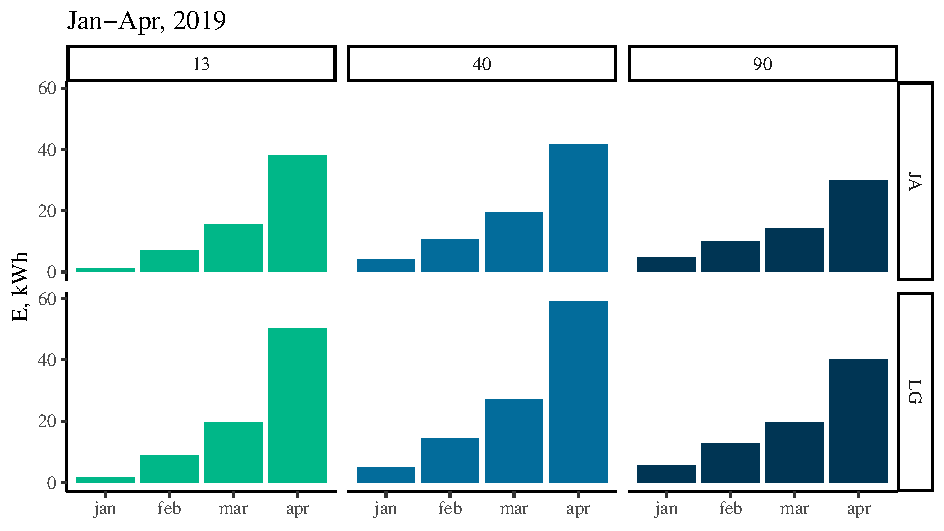
\includegraphics[width=\linewidth]{figures/results/jan_all_deg.pdf}
    \caption{D virzienā vērsto saules paneļu saražotā enerģija atkarībā no leņķa un saules paneļu tipa}
    \label{fig:ja_deg}
\end{figure}
\begin{figure}[h]
    \centering
    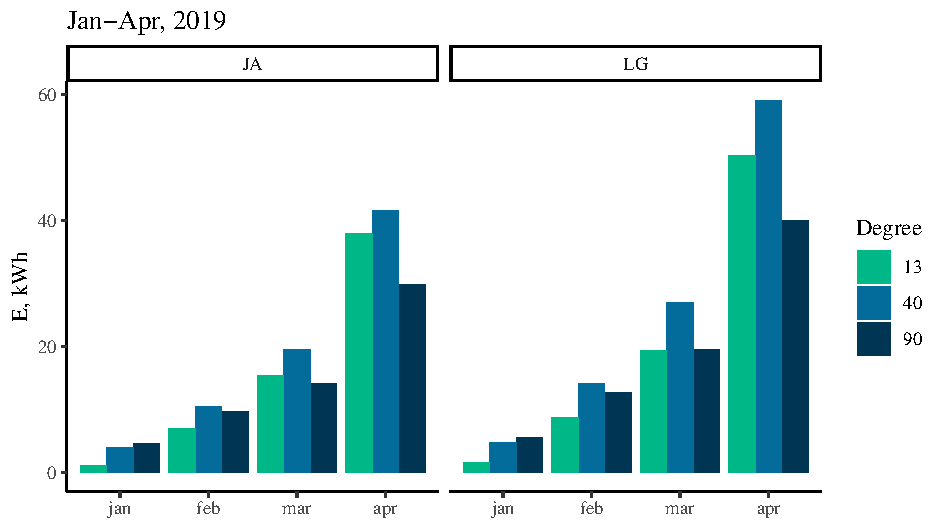
\includegraphics[width=\linewidth]{figures/results/degType.pdf}
    \caption{D virzienā vērsto saules paneļu saražotā enerģija atkarībā no leņķa un saules paneļu tipa}
    \label{fig:lg_ja_deg}
\end{figure}

\subsection{Saules paneļa virziena ietekme uz ražīgumu}
Dienvidi ir visražīgākais virziens, tad austrumi, tad rietumi.
\begin{figure}[h]
    \centering
    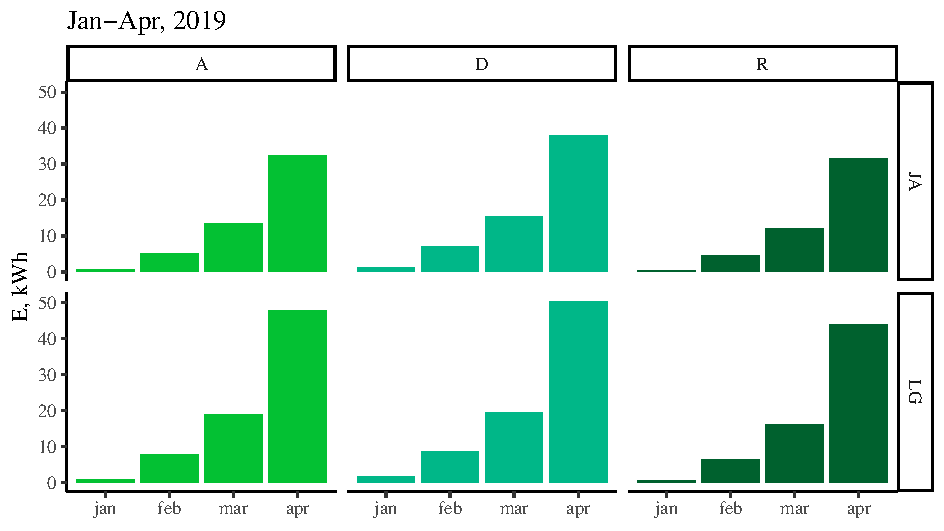
\includegraphics[width=\linewidth]{figures/results/jan_all_dir.pdf}
    \caption{13 grādu leņķī vērsto saules paneļu atkarība no virziena un saules paneļu tipa}
    \label{fig:ja_dir}
\end{figure}

\begin{figure}[h]
    \centering
    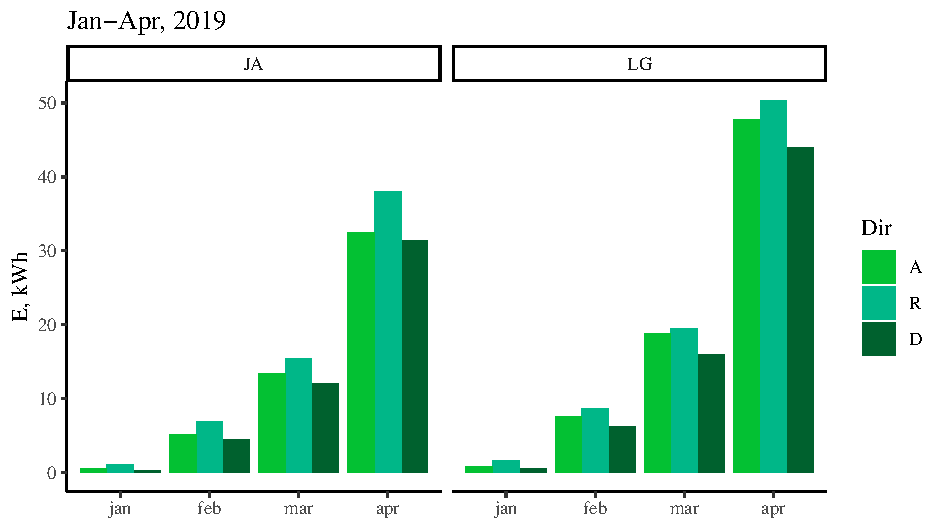
\includegraphics[width=\linewidth]{figures/results/dirType.pdf}
    \caption{13 grādu leņķī vērsto saules paneļu atkarība no virziena un saules paneļu tipa}
    \label{fig:lg_ja_dir}
\end{figure}

\subsection{Saules paneļa leņķa un virziena ietekme uz dienā saražotās enerģījas sadalījumu}
Kā redzams \ref{fig:feb_ar}, \ref{fig:mar_ar}, \ref{fig:apr_ar}. att., eksperimentāli noteiktais dienas sadalījums sakrīt ar teorētiski prognozēto \ref{fig:cos-theta}.att.

\begin{figure}[h]
    \centering
    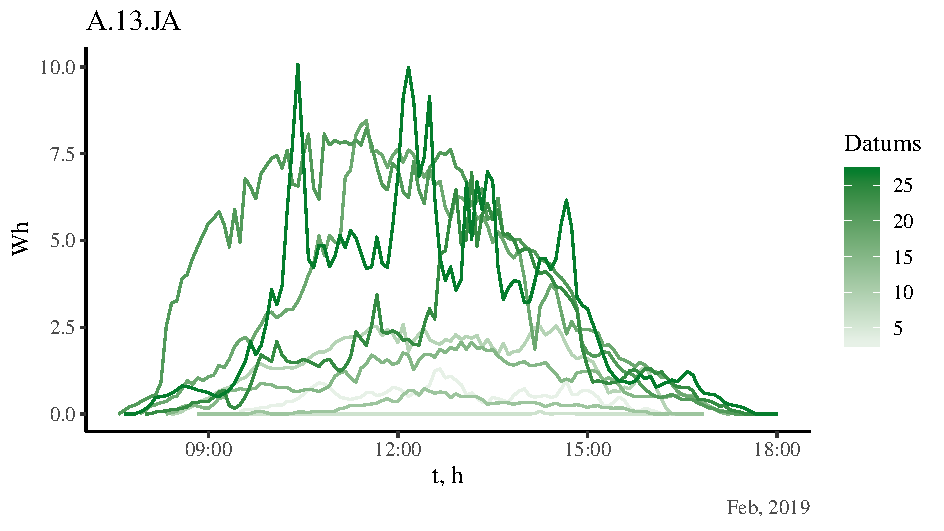
\includegraphics[width=\linewidth]{figures/sol_day/feb_A13JA.pdf}
    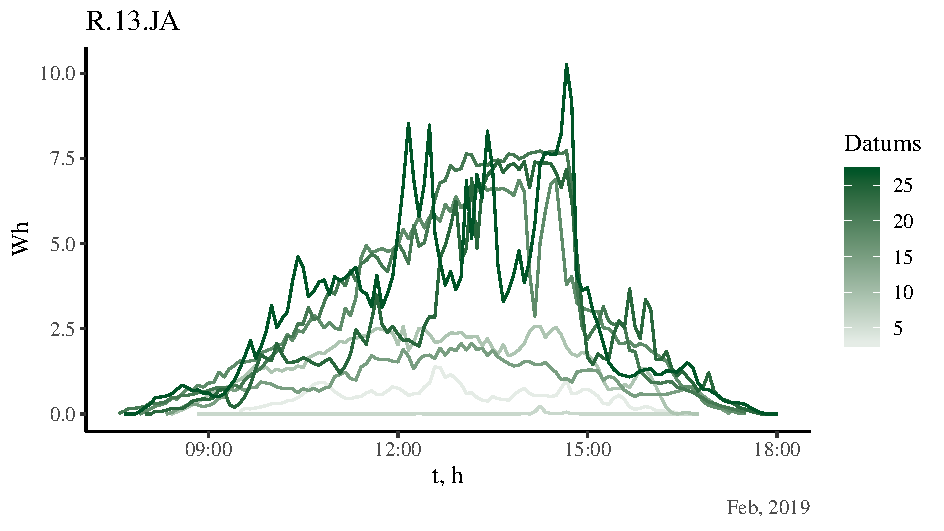
\includegraphics[width=\linewidth]{figures/sol_day/feb_R13JA.pdf}
    \caption{A un R virzienu saules paneļu 5 minūtēs vidējotu Wh dienas sadalījumi februārī}
    \label{fig:feb_ar}
\end{figure}

\begin{figure}[h]
    \centering
    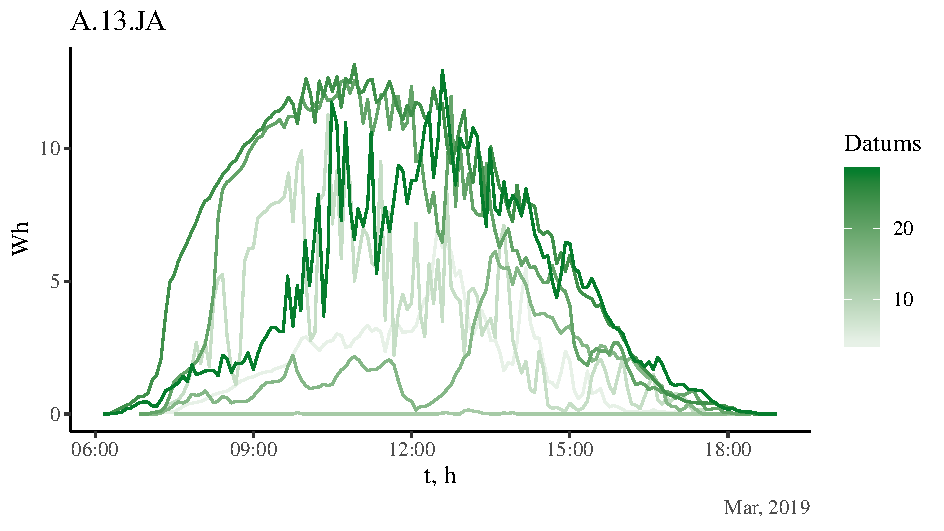
\includegraphics[width=\linewidth]{figures/sol_day/mar_A13JA.pdf}
    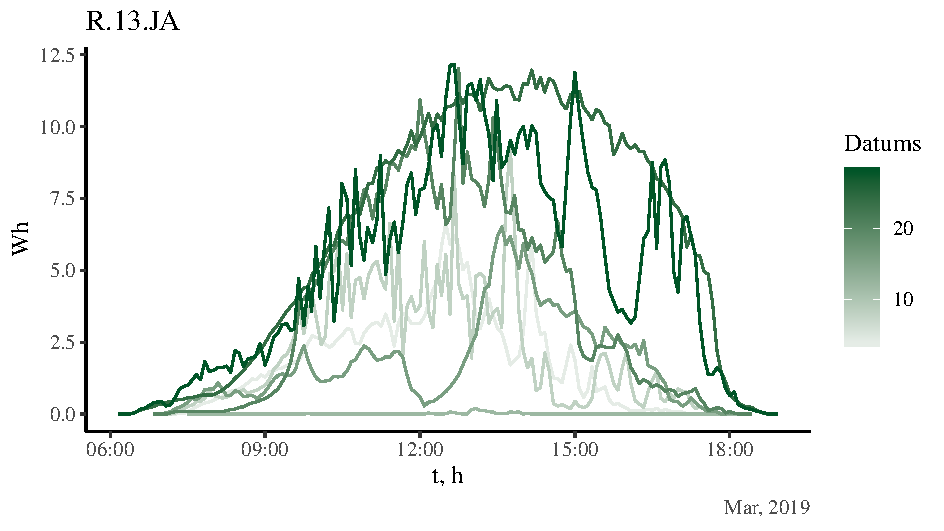
\includegraphics[width=\linewidth]{figures/sol_day/mar_R13JA.pdf}
    \caption{A un R virzienu saules paneļu 5 minūtēs vidējotu Wh dienas sadalījumi martā}
    \label{fig:mar_ar}
\end{figure}

\begin{figure}[h]
    \centering
    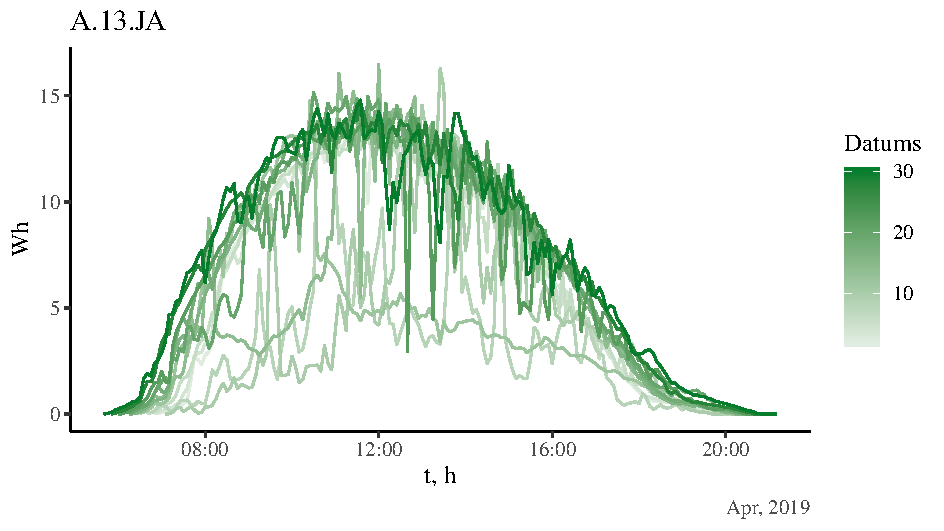
\includegraphics[width=\linewidth]{figures/sol_day/apr_A13JA.pdf}
    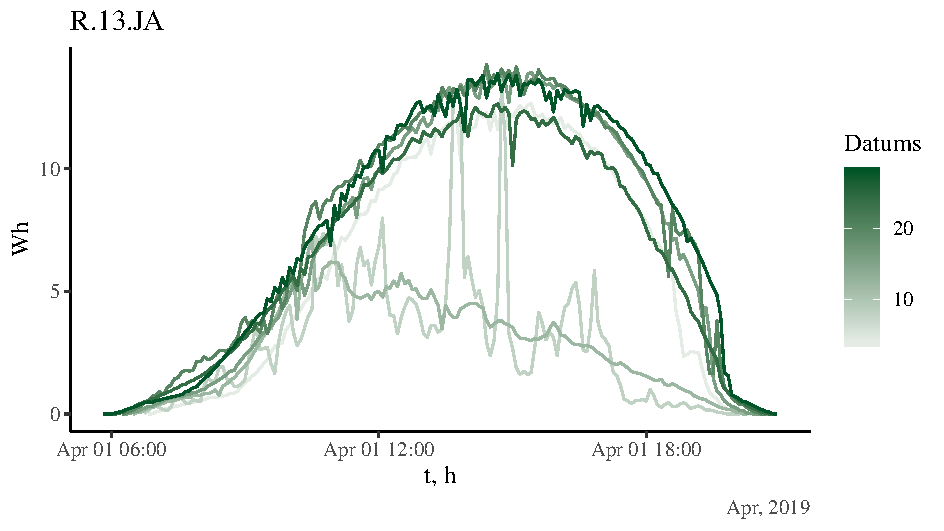
\includegraphics[width=\linewidth]{figures/sol_day/apr_R13JA.pdf}
    \caption{A un R virzienu saules paneļu 5 minūtēs vidējotu Wh dienas sadalījumi aprīlī}
    \label{fig:apr_ar}
\end{figure}

% \begin{figure}[h]
%     \centering
%     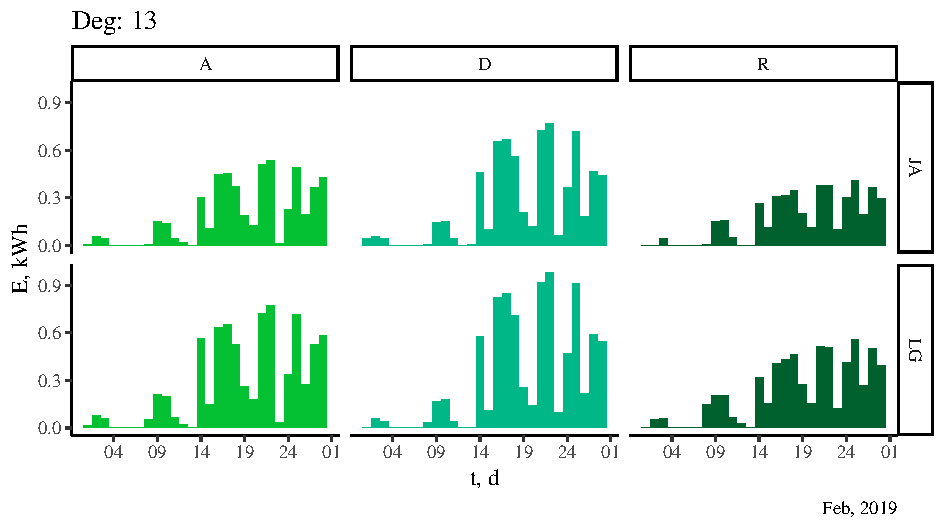
\includegraphics[width=\linewidth]{figures/sol_month/feb_Dir_d.pdf}
%     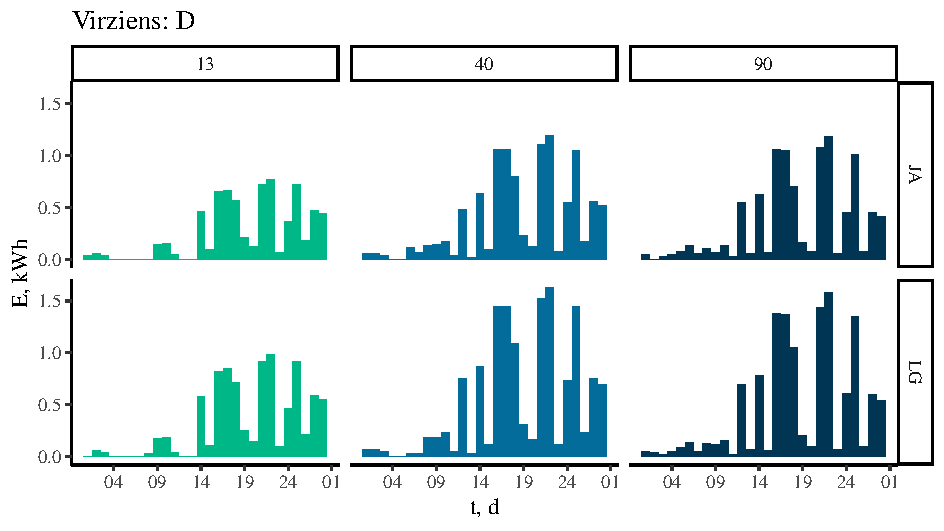
\includegraphics[width=\linewidth]{figures/sol_month/feb_Deg_d.pdf}
%     \caption{Saules paneļu saražotā enerģija atkarībā no virziena un leņķa februārī}
%     \label{fig:feb_degDir}
% \end{figure}

% \begin{figure}[h]
%     \centering
%     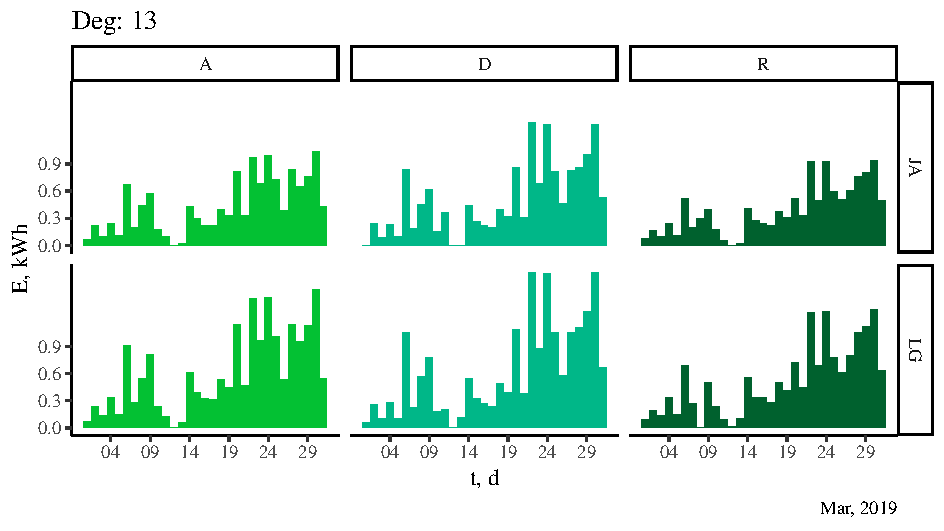
\includegraphics[width=\linewidth]{figures/sol_month/mar_Dir_d.pdf}
%     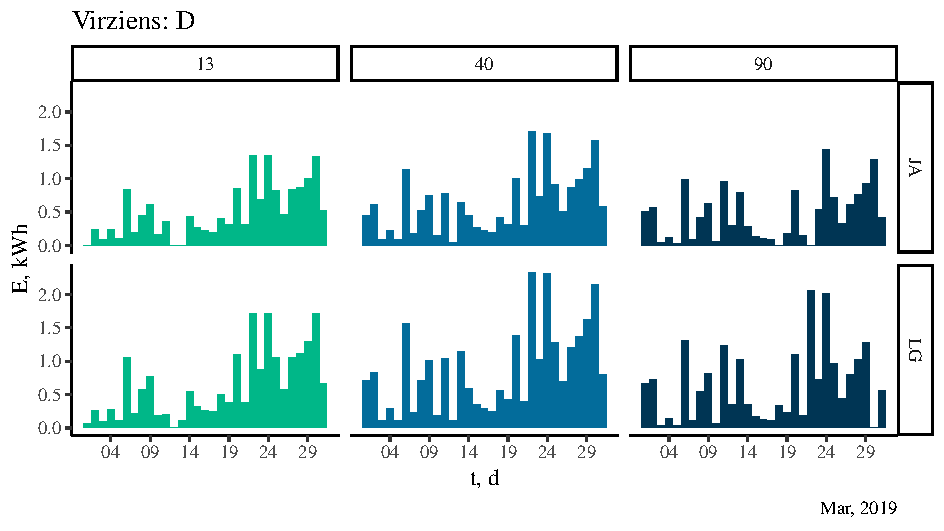
\includegraphics[width=\linewidth]{figures/sol_month/mar_Deg_d.pdf}
%     \caption{Saules paneļu saražotā enerģija atkarībā no virziena un leņķa martā}
%     \label{fig:mar_degDir}
% \end{figure}

% \begin{figure}[h]
%     \centering
%     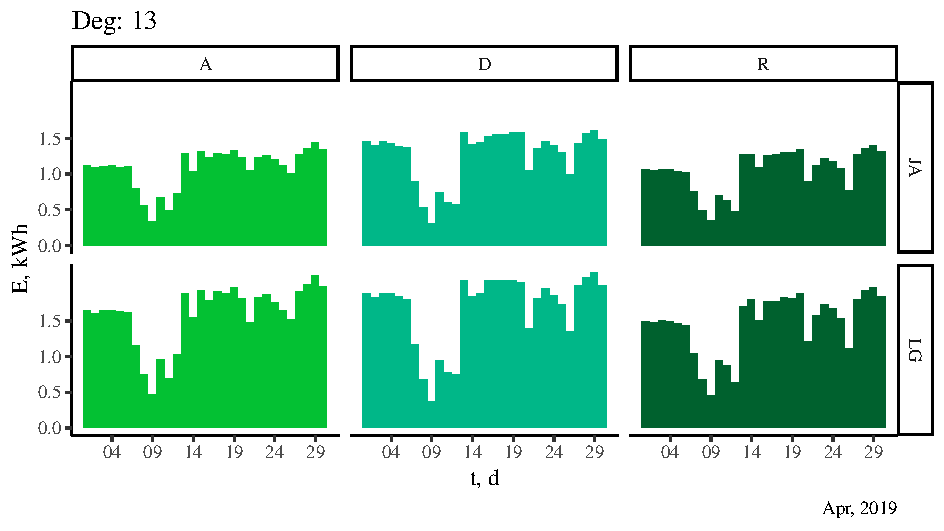
\includegraphics[width=\linewidth]{figures/sol_month/apr_Dir_d.pdf}
%     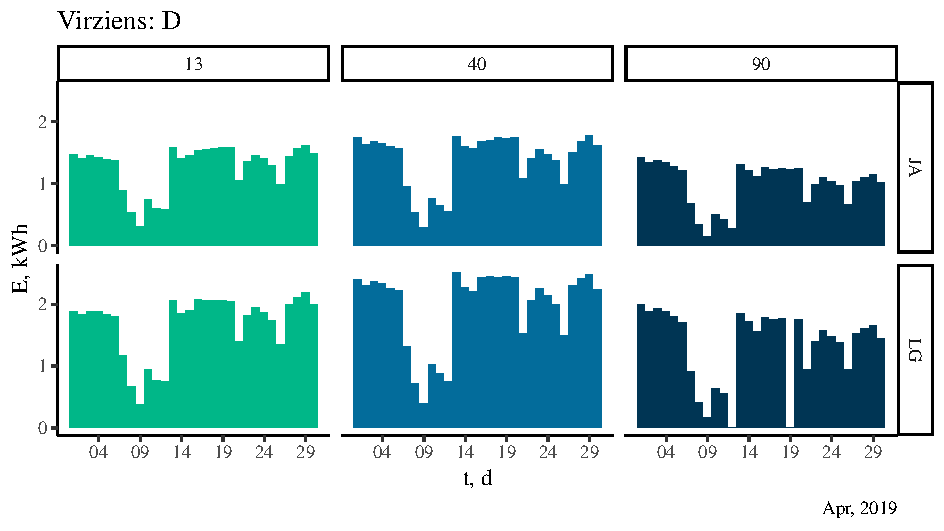
\includegraphics[width=\linewidth]{figures/sol_month/apr_Deg_d.pdf}
%     \caption{Saules paneļu saražotā enerģija atkarībā no virziena un leņķa aprīlī}
%     \label{fig:apr_degDir}
% \end{figure}

\subsection{Gada mēneša ietekme uz ražīgumu} % label chapter un atsaukties pirmajā apakšnodaļā uz šo
Pēc \ref{fig:jan_sum}, \ref{fig:feb_sun}, \ref{fig:apr_sum}, \ref{fig:apr_sum}. att., tiek izdarīti secinājumi par saules paneļu ražīguma atkarību no gada mēneša. Janvārī visražīgākais panelis ir D.90, otrs ražīgākais - D.40, kas atbilst janvārim raksturīgajai Saules diennakts kustībai -- zemu pie horzionta. \ref{fig:feb_sun}. att. redzams, ka februārī D.40 kļūst ražīgāks nekā D.90, tāpat redzams, ka mazāku leņķu paneļi - R.13 un A.13 ir palielinājuši ražīgumu. Šī tendence turpinās arī marta un aprīļa mēnešos.

\begin{figure}[h]
    \centering
    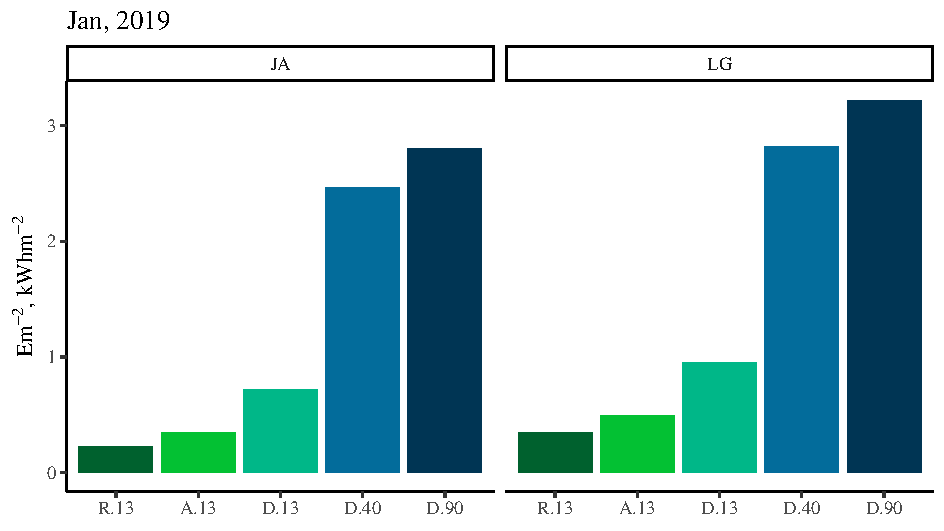
\includegraphics[width=\linewidth]{figures/sol_month/jan_m_m2.pdf}
    \caption{Saules paneļu saražotā enerģija janvārī}
    \label{fig:jan_sum}
\end{figure}

\begin{figure}[h]
    \centering
    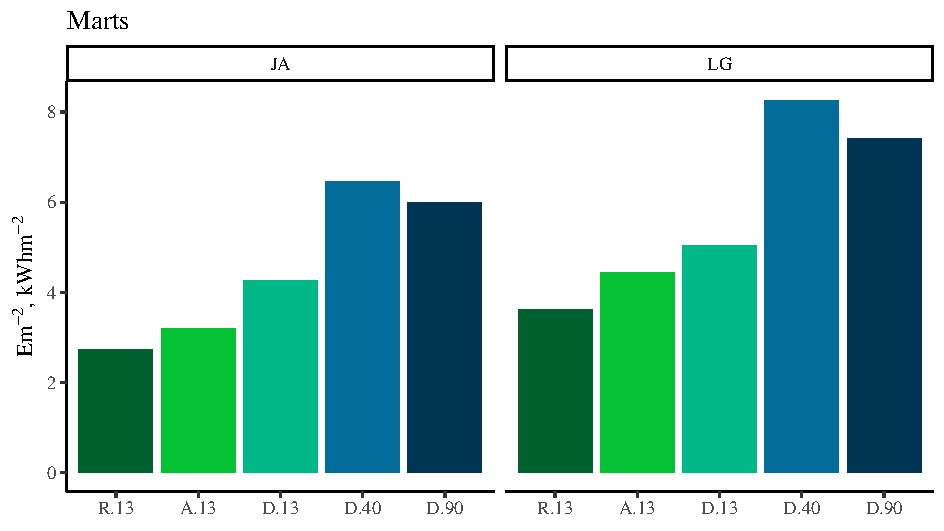
\includegraphics[width=\linewidth]{figures/sol_month/feb_m_m2.pdf}
    \caption{Saules paneļu saražotā enerģija februārī}
    \label{fig:feb_sum}
\end{figure}

\begin{figure}[h]
    \centering
    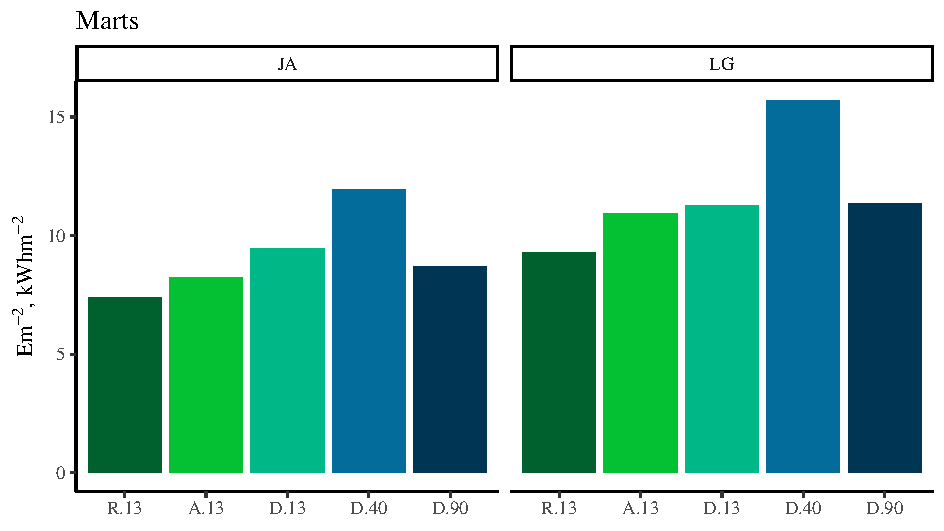
\includegraphics[width=\linewidth]{figures/sol_month/mar_m_m2.pdf}
    \caption{Saules paneļu saražotā enerģija martā}
    \label{fig:mar_sum}
\end{figure}

\begin{figure}[h]
    \centering
    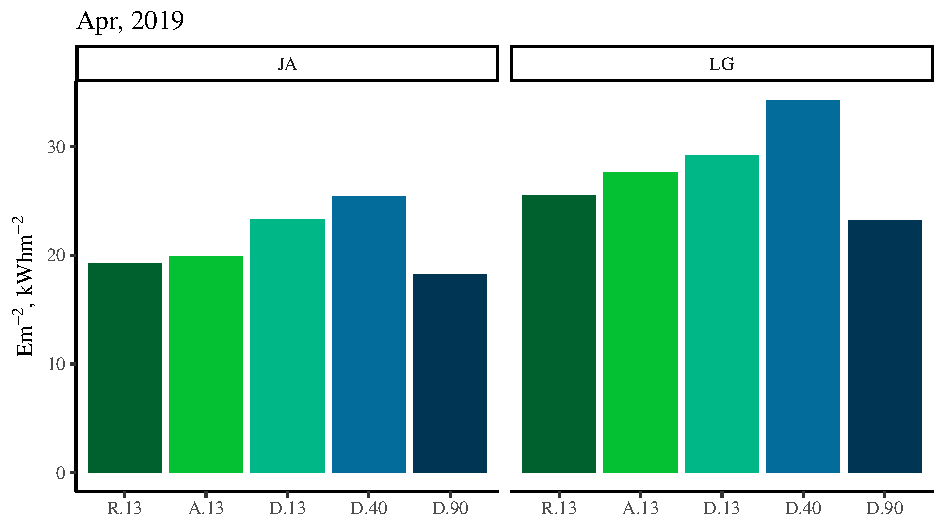
\includegraphics[width=\linewidth]{figures/sol_month/apr_m_m2.pdf}
    \caption{Saules paneļu saražotā enerģija aprīlī}
    \label{fig:apr_sum}
\end{figure}